%i primi parametri sono relativi alle dimensioni del carattere
%ed alla tipologia di pagina. Potete scegliere tra
%'10pt', '11pt' and '12pt', per la pagina 'a4paper', 'letterpaper', 'a5paper', %'legalpaper', 'executivepaper' o 'landscape')
\documentclass[10pt,a4paper,italian]{moderncv}
 
% lo stile del nostro curriculum
% come vedete ho scelto classic ma potete scegliere
% 'moderncv' 'casual' (si default),'classic', 'oldstyle' o 'banking'
% e i colori 'blu', 'orange', 'green', 'red', 'purple', 'grey' o 'black'
\moderncvtheme[blue]{classic}
 
% alcuni pacchetti standard
\usepackage[latin1]{inputenx}
\usepackage[T1]{fontenc}

\usepackage{graphicx}
\usepackage{epstopdf}
\usepackage[italian]{babel}
\usepackage[scale=0.8,top=1cm, bottom=2cm]{geometry}
 
% queste 2 righe servono per allargare la colonna di sinistra
\setlength{\hintscolumnwidth}{4cm}
\AtBeginDocument{\recomputelengths}
\usepackage{bibentry}
\usepackage{url}

 
%% altri pacchetti standard
%\usepackage{hyperref}
%\hypersetup{colorlinks=true}

 
% aggiungo la numerazione delle pagine (spesso inutile)
% obbligatorio se si usa hyperref (bug)
\pagenumbering{arabic}
 
% Dati personali
\firstname{Ivan}
\familyname{Bortolin}
\title{Curriculum Vitae}
\address{Omissis}{omissis}
\mobile{+39\,555\,207207}
% la mail ed il sito web avranno il collegamento multimediale
% all'interno del pdf
\email{ivan.bortolin@gmail.it}
\homepage{www.ivanbortolin.it}
% io ho omesso la foto, ma se voi la volete inserire basta
%aggiungerla nella cartella e mettere il nome del file
%\photo[100pt][0.6pt]{nome_file}
 
% da qui comincia il documento
\begin{document}
\maketitle
 
% per non far comparire i numeri di pagina
\pagestyle{empty}
 
% con il comando \sectio andiamo a creare delle sezioni nel documento e potremo
% nominarle come più ci aggrada nonché spostarle all'interno del CV in
% base alle nostre esigenze e stile
\section{Informazioni personali}
% per aggiungere voci nelle varie sezioni basta dare il comando
% \cvline {il_mio_testo}{il_mio_testo}
\cvline{nome}{Ivan}
\cvline{cognome}{Bortolin}
\cvline{sesso}{maschile}
\cvline{luogo e data di nascita}{Pordenone, 01 Maggio 1984}
\cvline{nazionalità}{italiana}
\cvline{stato civile}{celibe}
\cvline{patente di guida}{cat. B, conseguita il 01 Ottobre 2002}
\cvline{patente nautica}{abilitazione vela e motore senza limiti dalla costa, conseguita il 10 Maggio 2003}
 
\section{Titoli di studio}
 
\cvline{2003}{\textbf{Diploma di Maturità Classica}\newline
presso Scuola Navale Militare "Francesco Morosini" Venezia con votoazione 83/100}
 
\cvline{2012}{\textbf{Laureando}\newline
in Ingegneria Elettronica, curriculum professionalizzante in Automazione Industriale, presso l'Università degli studi di Udine}
 
\cvline{}{\textbf{Tesi di laurea}\newline
Progettazione e realizzazione di una stampante 3D di grandi dimensione per la prototipazione rapida.
Le competenze approfondite durante le fasi di sviluppo sono: \newline
- programmazione scheda elettronica "Arduino" \newline
- funzionamento e controllo del processo di estrusione di materie plastiche
\newline - controllo moti a passo}
 
\section{Conoscenze informatiche}
\cvline{}{Conoscenza avanzata di tutte le applicazioni per ufficio più comuni}
 
% voi aggiungete tutte le voci che ritenete opportune
% nel caso abbiate delle pubblicazioni, dopo aver creato l'opportuno file .bib
% NB: io ho disbilitato questi comandi
%\nocite{*}
%\bibliographystyle{plain}
%\bibliography{nome_file.bib}   
 
% Ora ci resta solo che inserire la liberatoria per la privacy
% Io ho scannerizzato direttamente la mia firma e l'ho inserita come
% immagine. Nel caso vogliate mettere dei puntini e firmare personalmente
% ogni CV dopo il “in fede” scrivere \makebox[9cm]{\dotfill}
\vspace{\fill}
{\footnotesize\noindent
Il sottoscritto è a conoscenza che, ai sensi dell'art. 26 della legge 15/68, le dichiarazioni mendaci, la falsità negli atti e l'uso di atti falsi sono puniti ai sensi del codice penale e delle leggi speciali. Inoltre, il sottoscritto autorizza al trattamento dei dati personali, in conformità alle disposizioni della legge sulla privacy  (D.L.196/03).}
\vspace*{0.8cm}\\
Udine, \today\hfill In fede: \makebox[6cm]{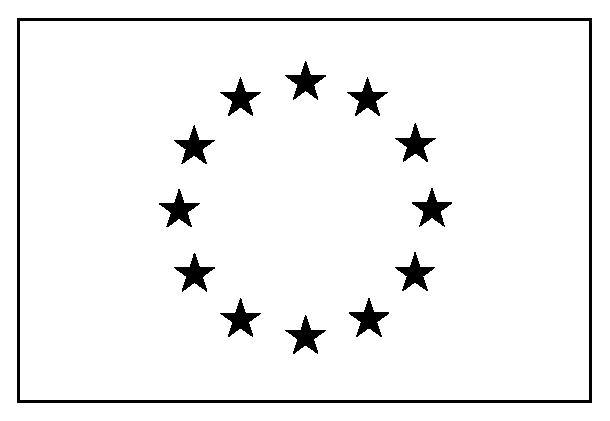
\includegraphics[scale=1]{picture.eps} }
%%per scalare la grandezza dell'immagine di firma, variate il parametro “scale”
\end{document}
